\chapter{人工データ実験}
\section{シミュレーション}
ニューロン集団のカルシウムイメージングデータをシミュレーションによって作り,解析手法を評価する.
シミュレーションでは1)ニューロンのネットワーク構造を作成し,2)スパイクのシミュレーションを行い,3)蛍光強度の観測データに変換する.
\subsection{ネットワーク構造}
シミュレーションに用いるニューロンの個数を$N$として,ニューロンのネットワーク構造を$S \in {0, 1}^{N \times N}$とする.
$s_{ij}$はニューロン$i$からニューロン$j$へ活動電位が伝わるかを表している.
本節では$S$の作り方を説明する.

ニューロンのネットワーク構造にはsmall world network\cite{Watts1998}を用いる.
Small world networkはノード数,張り替え確率,初期次数を決めることによってネットワークを作成するアルゴリズムである.
初期次数は,ニューロンが平均何個のニューロンとシナプス結合を持つかという変数である.
張り替え確率は,初期次数によって作成された規則的なグラフのエッジをランダムに張り替える確率である.
そのため,エッジのうち何割が遠くのニューロンとつながっているかを表す変数である.

実際のニューロンをsmall world networkによって表すために,初期次数と張り替え確率を実データから決める.
今回はこの値はニューロンのコネクションの割合と相互のコネクションの割合から決める.
興奮性ニューロン同士の6.7\%であり,そのうち双方向のコネクションの割合は24\%である\cite{Jouhanneau2015}.
発達中マウスの興奮性ニューロンから抑制性ニューロンへのコネクティビティと抑制性ニューロンから興奮性ニューロンへのコネクティビティはどちらも78\%であった\cite{Holmgren2003}.
成熟したマウスではより少ないと思われるが,データが見つからなかったため,40\%とした.
相互のコネクションの割合がランダムにエッジを作るよりも高いのは,近いニューロンにコネクションが作られやすいからだと考えられる.
これらのデータを実現するように初期次数と張り替え確率を調整した.
用いたパラメータを\Tabref{tab:parameter1}に示す.
抑制性ニューロン同士のコネクティビティは分からないため,興奮性ニューロンと同じにしている.

\begin{table}[htb]
  \center
  \begin{tabular}{|c|cc|} \hline
    結合の種類 & 初期次数 & 張り替え確率 \\ \hline
		同種類のニューロン間 & $0.0335 N$ & $0.3$ \\
		興奮性ニューロンと抑制性ニューロン間 & $0.2N$ & $0.3$\\ \hline
  \end{tabular}
  \caption{ネットワーク構造のパラメータ}
  \label{tab:parameter1}
\end{table}

実際のネットワーク構造の作り方を説明する.
ネットワーク構造は興奮性ニューロン同士の結合,抑制性ニューロン同士の結合,興奮性ニューロンと抑制性ニューロン間の結合の3つに分けて作成する.
まず,全ニューロンのうち抑制性ニューロンと興奮性ニューロンのインデックスを決めておく.
全てのニューロンについて\Tabref{tab:parameter1}に従ってネットワークを作成し,それぞれに対応する隣接行列の上三角または下三角行列を取り出して結合する.
作成したいのは向きのある有向グラフなので,上三角行列と下三角行列を分けて作成する.

\subsection{スパイクシミュレーション}
スパイクのシミュレーションにIzhikevichモデル~\cite{Izhikevich2003}を用いる.
このモデルはHodgikin-Huxleyモデルをもとにしており,計算コストが低い.
Izhikevichモデルでは,あるニューロンの膜電位が閾値を超えると発火したとみなし,あらかじめ定義したニューロンのネットワーク構造に従って結合を持つニューロンの膜電位を上昇させる.
このシミュレーションで設定しなければいけないのは,個々のニューロンの特徴パラメータ,重み付きのネットワーク構造,外部からのランダムな入力である.

まず,個々のニューロンの特徴パラメータについて説明する.
このモデルではニューロンごとに4つのパラメータを設定する必要があり,そのパラメータでニューロンを特徴づける.
本論文では興奮性ニューロンにはregular spiking neurons,抑制性ニューロンにはfast spiking neuronsを用いる.
それらのパラメータを~\Tabref{tab:parameter2}に示す.
ただし,$r_e$と$r_i$は0から1の一様分布に従う確率変数である.

\begin{table}[htb]
  \center
  \begin{tabular}{|c|cccc|} \hline
    ニューロンの種類 & a & b & c & d \\ \hline
    興奮性ニューロン & 0.02 & 0.2 & $-65 + 15 r_e^2$ & $8 - 6r_e^2$ \\
    抑制性ニューロン & $0.02 + 0.08r_i$ & $0.25 - 0.05 r_i$ & -65 & 2 \\ \hline
  \end{tabular}
  \caption{Izhikevichモデルのパラメータ}
  \label{tab:parameter2}
\end{table}

次に,重み付きのネットワーク構造$W \in \mathbb{R}^{I \times I}$について説明する.
ニューロン$i$から$j$へ結合があった場合,$w_{ij}$はニューロン$i$が発火した時にニューロン$j$の膜電位をどれだけ上昇させるかという数値である.
$W$は,前節で作成した$S$の非ゼロ要素を数値で置き換えることで作成する.
興奮性ニューロンからの結合は一様分布$U(0, 0.5)$からサンプルし,抑制性ニューロンからの結合は一様分布$U(-2,0)$からサンプルする.
\begin{align}
	w_{ij} = \begin{cases}
		U(0,0.5) & (s_{ij} = 1 \ and \ i \in \ excitatory \ neuron) \\
		U(-2,0) & (s_{ij} = 1 \ and \ i \in \ inhibitory\  neuron) \\
		0 & (s_{ij} = 0)
  \end{cases}
	\label{eq:W}
\end{align}

最後に外部からのランダムな入力について説明する.
ニューロンには観測範囲外からの入力がある(以降,外部入力とする).
そのため,シミュレーション中も外部からの電位を乱数としてニューロンの電位に足す.
本論文では,ニューロンの活動も外部入力の大きさで表現する.
活動していない興奮性ニューロンと抑制性ニューロンにはそれぞれ,$\mathcal{N}(0,5)$と$\mathcal{N}(0,2)$に従う乱数を足す.
活動している興奮性ニューロンと抑制性ニューロンにはそれぞれ,$\mathcal{N}(1,5)$と$\mathcal{N}(0.4,2)$に従う乱数を足す.
これらを\Tabref{tab:parameter3}に示す.
活動していないニューロンへの外部入力は\cite{Izhikevich2003}で用いられていたものを採用した.
ただし,興奮性ニューロンの活動時の外部入力は変化させた実験もある.

\begin{table}[htb]
  \center
  \begin{tabular}{|c|cc|} \hline
    ニューロンの種類 & 活動時の外部入力 & 活動していない時の外部入力 \\ \hline
		興奮性ニューロン & $\mathcal{N}(0.8,3)$ & $\mathcal{N}(0, 5)$ \\
		抑制性ニューロン & $\mathcal{N}(0.4, 0.1)$ & $\mathcal{N}(0, 2)$ \\ \hline
  \end{tabular}
  \caption{シミュレーションに用いる外部入力の値}
  \label{tab:parameter3}
\end{table}

本論文では同時に活動するニューロンを推定するのが目的の1つである.
ある時間帯にあるニューロングループが活動する時,そのニューロングループには平均値を上げた外部入力を足し,それ以外のニューロンには平均$0$の外部入力を足す.
こうすることで,ニューロングループの活動のみ上がる(つまり蛍光強度が上がる).
実際の脳でもこのように外部からの入力によってニューロンの活動を制御していると考えられる.
あるニューロングループを活動させるには,そのグループのハブとなるニューロンにのみ強い外部入力を与える方法も考えられるが今回は採用しない.
なぜなら,ネットワーク構造をかなり工夫しないと実現できないためである.

実際にマウスのニューロンの発火頻度がどれくらいなのか\cite{Watson2016}を元に\Tabref{tab:spike-frequency}に示す.
\begin{table}[htb]
  \center
  \begin{tabular}{|c|ccc|} \hline
    ニューロンの種類 & 覚醒時(Hz) & ノンレム睡眠時(Hz) & レム睡眠時(Hz) \\ \hline
		興奮性ニューロン & $0.76 \pm 1.53$ & $0.69 \pm 0.86$ & $0.88 \pm 1.33$ \\
		抑制性ニューロン & $5.59 \pm 7.25$ & $4.69 \pm 5.62$ & $4.25 \pm 9.43$ \\ \hline
  \end{tabular}
  \caption{ニューロンごとの発火頻度の中央値}
  \label{tab:spike-frequency}
\end{table}

\subsection{カルシウムイメージングモデル}
スパイクデータからカルシウムイオン濃度を計算する~\cite{Vogelstein2009}のモデルを用いる:
\begin{equation}
  [Ca^{2+}]_{i,t} - [Ca^{2+}]_{i,t-1} = - \frac{\Delta}{\tau}([Ca^{2+}]_{i,t-1} - [Ca^{2+}]_b) + An_{i,t} + \sigma_c \sqrt{\Delta} \epsilon_{i,t},
  \label{eq:calcium}
\end{equation}
ただし,$[Ca^{2+}]_{i,t}$をニューロン$i$の時刻$t$でのカルシウムイオン濃度,$[Ca^{2+}]_b$をカルシウムイオン濃度のベースライン,$\Delta$を時間幅,$\tau$は時定数,$A$は1つのスパイクでのカルシウムイオン濃度の上がり幅,$n_{i,t} \in \{0,1\}$はニューロン$i$の時刻$t$でのスパイク,$\sigma_c$はノイズの分散,$\epsilon_{i,t}$は標準正規分布に従う確率変数である.
この人工データではsaturationは考えないこととする.

次に,同論文のモデルを使ってカルシウムイオン濃度$[Ca^{2+}]_{i,t}$をカルシウムイメージングで計測される蛍光強度$F_{i,t}$に変換する:
\begin{equation}
	F_{i,t} = \alpha[Ca^{2+}]_{i,t} + \beta + \sigma_F \epsilon_{i,t},
  \label{eq:intensity}
\end{equation}
$\alpha$は強度,$\beta$はバイアス,$\sigma_F$はノイズの分散である.

\Tabref{tab:parameter2}に使用したパラメータを示す.

\begin{table}[htb]
  \center
  \begin{tabular}{|cccccccc|} \hline
    $[Ca^{2+}]_b$ & $\Delta$ & $\tau$ & $A$ & $\sigma_c$ & $\alpha$ & $\beta$ & $\sigma_F$ \\ \hline
    0.1 & 0.001 & 0.5 & 5.0 & 1.0 & 1.0 & 0 & 1.0 \\ \hline
  \end{tabular}
  \caption{カルシウムイメージングモデルでのパラメータ}
  \label{tab:parameter2}
\end{table}

\subsection{観測モデル}
実データは8 Hzでサンプリングされたデータなので,シミュレーションした蛍光強度を8 Hzで足し合わせる:
\begin{equation}
  x_{i,t'} = \sum_{t=1}^{125} F_{i,t},
  \label{eq:observation}
\end{equation}
ここで,$t'$はサンプリング後の時刻を表す.

上記の方法で作成した人工データ時系列と観測時系列をそれぞれ\Figref{fig:art}と\Figref{fig:dat}に示す.
\begin{figure}[htbp]
    \begin{minipage}{0.5\hsize}
			\begin{center}
					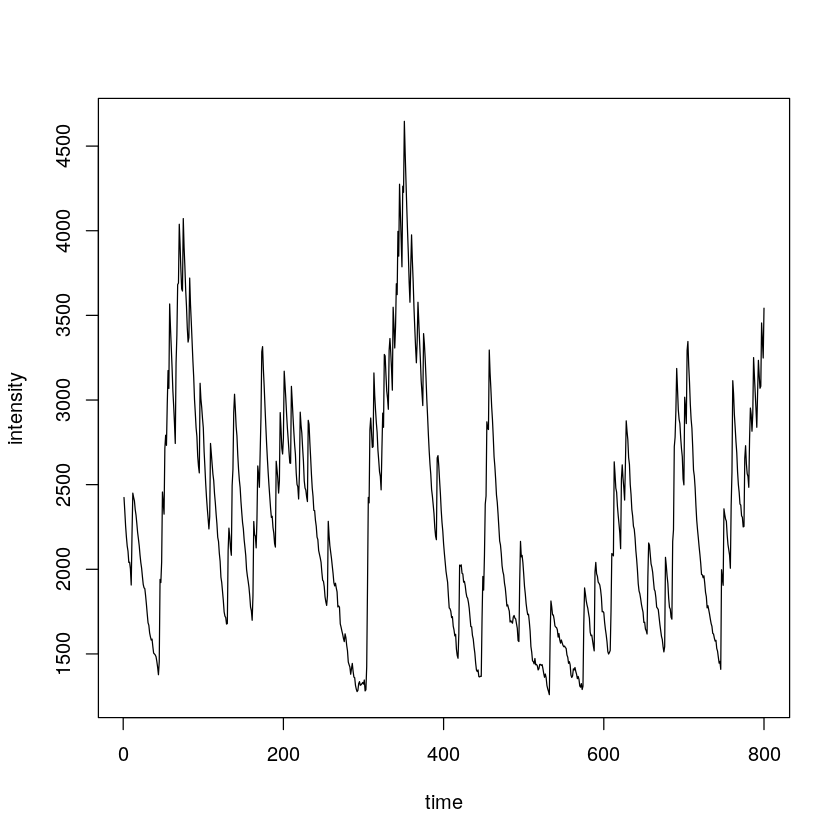
\includegraphics[width=\hsize]{artificial_data}
					\caption{1つのニューロンの人工時系列.}
					\label{fig:art}
			\end{center}
		\end{minipage}
    \begin{minipage}{0.5\hsize}
			\begin{center}
					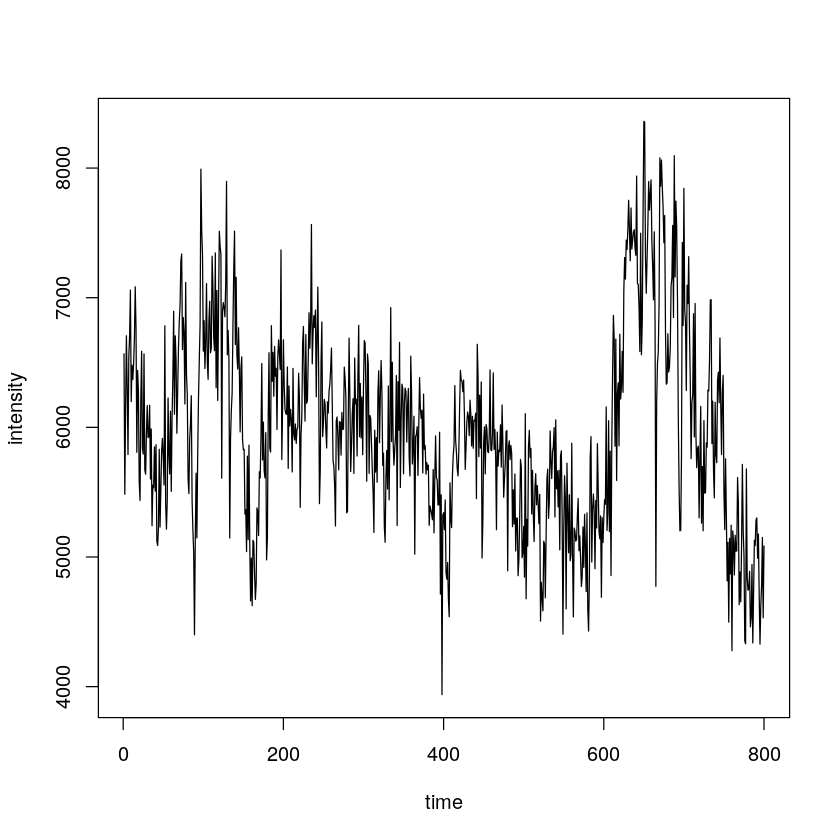
\includegraphics[width=\hsize]{real_data}
					\caption{1つのニューロンの観測時系列.}
					\label{fig:dat}
			\end{center}
		\end{minipage}
\end{figure}

\subsection{実験設定}
800個の興奮性ニューロンと200個の抑制性ニューロンについてネットワーク構造$S$を作成し,\eqref{eq:W}に従って重み付きネットワーク構造$W$を作成した.
$W$は全実験を通して固定である.

$W$を元にカルシウムイメージングのシミュレーションを行った.
1つのグループに所属するニューロン数は50〜200個とした.
グループが活動する時間は5sごとに変えた.
全1000個のニューロンのうち,解析に用いるのは固定された100個の興奮性ニューロンのみとする.

\begin{enumerate}
  \item ニューロンは1つのグループに必ず所属する
  \item ニューロンは1つのグループに所属するかグループに所属しない
  \item ニューロンは1つか2つのグループに必ず所属し,同じニューロンが所属しているグループ同士の活動は被らない
\end{enumerate}
% シミュレーション時間は470sで,そのうちの10sは安定のため解析から除外した.

\section{$A$の推定に関する結果}
本節では$A$の推定に関する結果について述べる.
実験は,5sごとに1つか2つのグループが活動するデータを105sシミュレーションさせた結果を用いた.
ただし,最初の5sはシミュレーション数値の安定性のため解析から除外した.

\subsection{$A$の一意性}
前章で述べた通り,NMFには一意性がないため$A$にも一意性がない.
1つの人工データについて初期値を変化させてNMFを行うと推定される$A$は同じではない.
$A$の上三角の要素について$1$と推定された頻度を調べる.
収束性と前章で述べたように寄与率が$D$の空間で取りうる値の範囲を狭めるため,$C$の行和を1とする制約を入れている.
$X$に正規化を加えなかった結果を\Figref{fig:without_scale_A}に,$X$に行和$1$の正規化を加えた結果を\Figref{fig:with_scale_A}に示す.
$X$に行和$1$の正規化を加えると,$D$の自由度は下がる.

\begin{figure}[htbp]
    \begin{minipage}{0.5\hsize}
			\begin{center}
					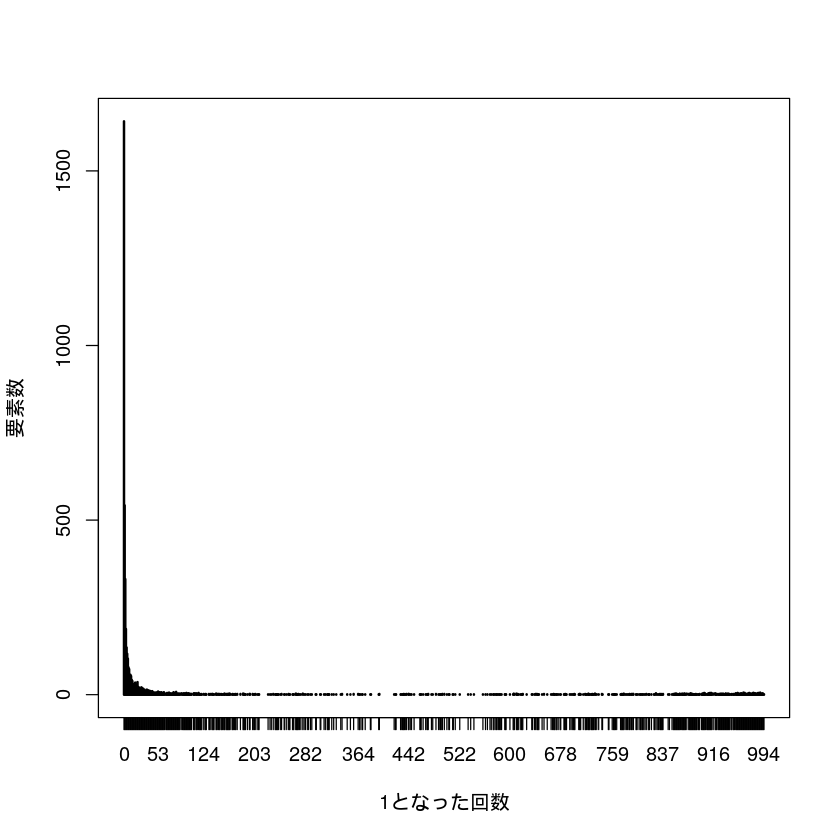
\includegraphics[width=\hsize]{without_scale_A}
					\caption{$X$を正規化せずに初期値を1000回変化させてNMFから$A$を推定し,各要素について$1$と推定された頻度をプロットした.}
					\label{fig:without_scale_A}
			\end{center}
		\end{minipage}
    \begin{minipage}{0.5\hsize}
			\begin{center}
					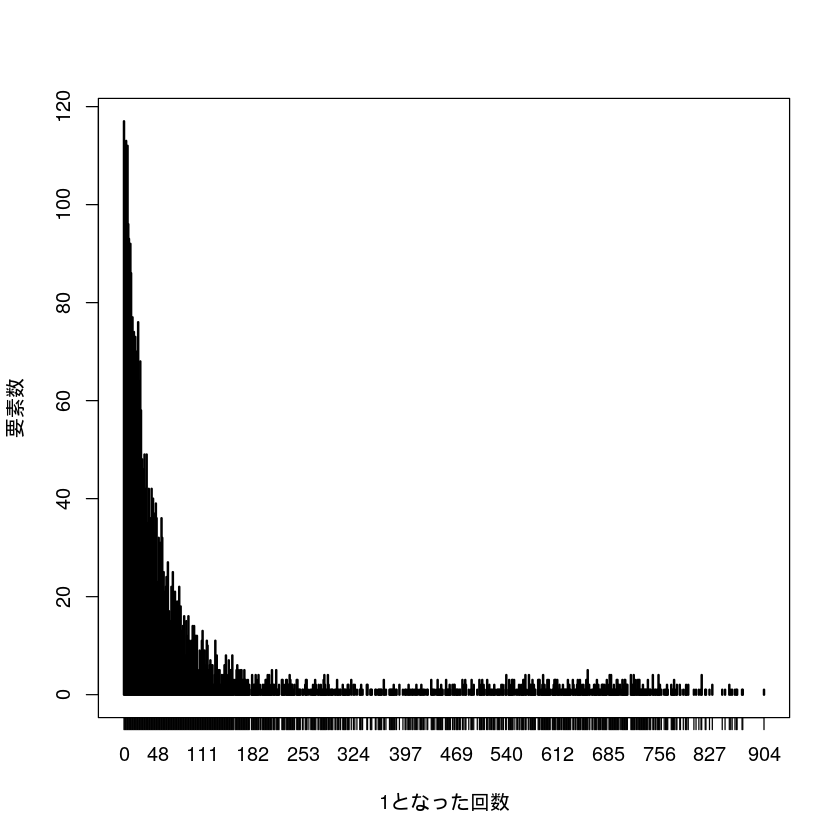
\includegraphics[width=\hsize]{with_scale_A}
					\caption{$X$を行和$1$で正規化して初期値を1000回変化させてNMFから$A$を推定し,各要素について$1$と推定された頻度をプロットした.}
					\label{fig:with_scale_A}
			\end{center}
		\end{minipage}
\end{figure}

$A$に一意性がある場合は,ある$A$の要素が$1$と推定される回数は$0$か$1000$になる.
結果より,そうなっていないので$A$に一意性がないのがわかる.
また,\Figref{fig:with_scale_A}より$X$を正規化した方がよりばらつきが大きくなっているのがわかる.
これは,正規化をしない方が$X$の中の大きな値に推定が引っ張られ,同じ局所解に落ちやすくなっているからだと考えられる.
また,この正規化の仕方は物理的には,ある期間にニューロンの活動の総和が一定であるという意味をもつ.
実際はそうではないので,今回の正規化の仕方はこの実験のみに留める.

\subsection{手法の比較}
NMF,PCA,ICA,logistic regression,glassoの性能の比較を行った.
Logistic regressionとglassoについては筆者の卒論を参照されたい.
どちらも時間窓をスライドさせてネットワークを行う.
今回の実験では時間窓を40,スライド幅を20とした.
Glassoのハイパーパラメータを$\rho = 0.3$とした.
一回でもエッジが張られたニューロン同士は同じグループとして推定量$A$と同じ行列を作成した.

PCAとICAはNMFと同じく一般化線形成分分析の手法\cite{Cichocki2009}である.
PCAとICAでは$D$に相当する行列でNMFと同じく推定量$A$を作成する.

2のタイプについて100種類のデータを生成し,$A$を閾値$0.5$で切って${0,1}^{I \times I}$の行列にした時のF1 scoreを比較した.
\begin{figure}[htbp]
    \begin{center}
        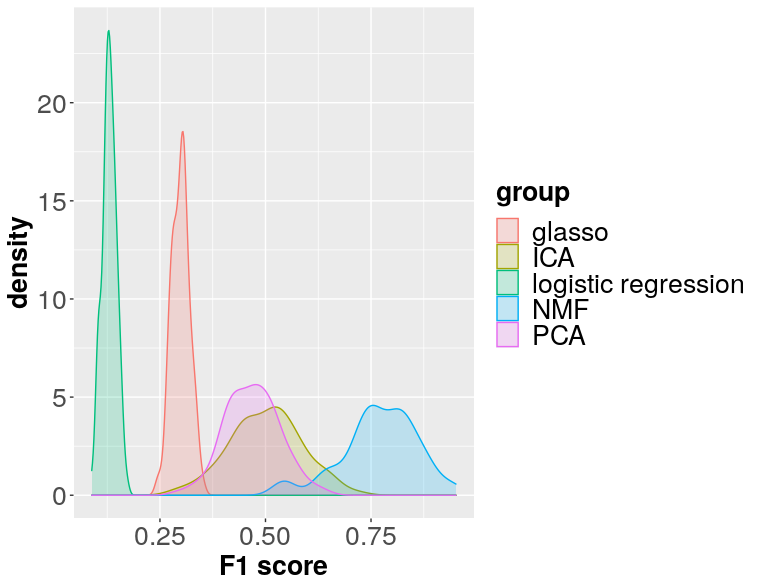
\includegraphics[width=0.5\linewidth]{compare-models}
        \caption{NMF,PCA,ICA,logistic regression,glassoのF1 scoreの密度分布}
        \label{fig:compare-models}
    \end{center}
\end{figure}
\Figref{fig:compare-models}より,NMFの精度が最も高いことが分かる.
NMFの非負制約がデータに合っているためだと思われる.
Glassoとlogistic regressionについてはニューロングループを推定するという実験設定はやや不利で合った.
各窓ごとのニューロンネットワークの活動を反映している可能性があるので悪い手法とはいえない.

% \subsection{推定へのネットワーク構造の影響}
% グループ推定へのネットワーク構造の影響を調べるために,1と2のネットワーク構造とグループについて100種類のデータを生成し,NMFの推定精度の比較を行った.
% 人工データは,近いニューロンほどつながりやすい性質をもつので,1の人工データの方がニューロン同士が同期して活動しやすいと思われる.
% ここで,2つのニューロンが同期するとは,一方のニューロンが発火してからごく短い間にもう一方のニューロンが発火する状態が続くことである.
% 実験結果を\Figref{fig:same-exc}~\ref{fig:diff-inh}に示す.
% \begin{figure}[htbp]
%     \begin{center}
%         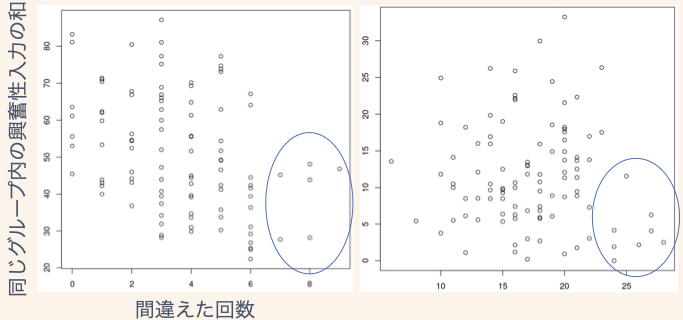
\includegraphics[width=\linewidth]{same-exc}
%         \caption{データ1と2について,ニューロンごとの間違えた回数と同じグループからの興奮性入力の和の関係}
%         \label{fig:same-exc}
%     \end{center}
% \end{figure}
% \begin{figure}[htbp]
%     \begin{center}
%       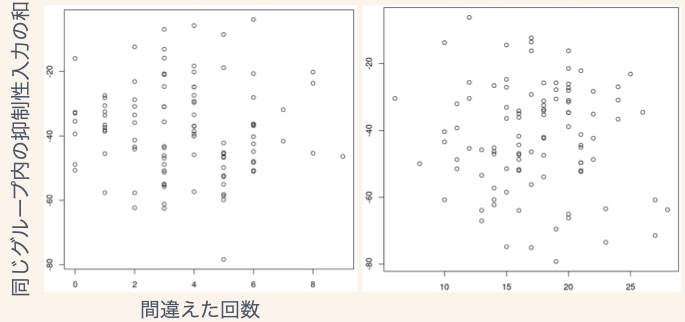
\includegraphics[width=\linewidth]{same-inh}
%         \caption{データ1と2について,ニューロンごとの間違えた回数と同じグループからの抑制性入力の和の関係}
%         \label{fig:same-inh}
%     \end{center}
% \end{figure}
% \begin{figure}[htbp]
%     \begin{center}
%         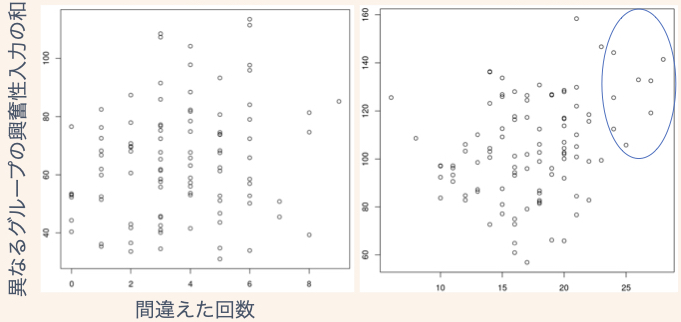
\includegraphics[width=\linewidth]{diff-exc}
%         \caption{データ1と2について,ニューロンごとの間違えた回数と異なるグループからの興奮性入力の和の関係}
%         \label{fig:diff-exc}
%     \end{center}
% \end{figure}
% \begin{figure}[htbp]
%     \begin{center}
%         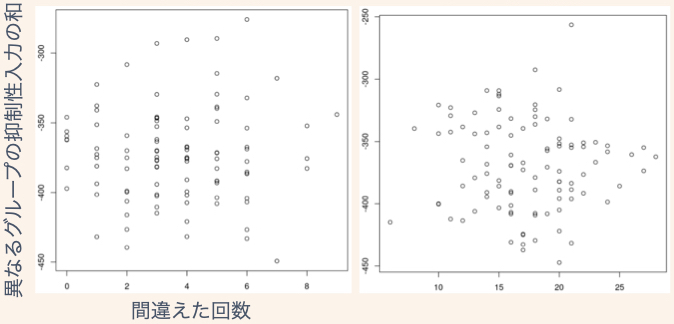
\includegraphics[width=\linewidth]{diff-inh}
%         \caption{データ1と2について,ニューロンごとの間違えた回数と異なるグループからの興奮性入力の和の関係}
%         \label{fig:diff-inh}
%     \end{center}
% \end{figure}
% \Figref{fig:same-inh},\Figref{fig:diff-inh}より,抑制性の入力は間違える回数には影響しないと思われる.
% \Figref{fig:same-exc}より,同じグループからの興奮性入力が小さいと間違えやすいと言える.
% \Figref{fig:diff-exc}より,データ2で間違える回数が多かったニューロンは異なるグループからの興奮性入力が大きかった.
% データ2ではデータ1よりも近いニューロンが異なるグループに所属する割合が多い.
% そのため,異なるグループからの興奮性入力と間違える回数の関係が強く出たと思われる.
% 
% 他にも推定へのネットワーク構造の影響の調査を試みたが,はっきりとした結果は得られなかった.

\subsection{モデル平均の有用性}
バギングの有用性を確認するために各人工データについて,1回NMFを行った結果,30回初期値を変えた結果,30回ブートストラップした結果のF1 scoreを~\Figref{fig:once-init-boot}に示す.
なお,NMFは20回初期値を変化させて再構成ごさが最小となる結果を1回の結果として用いた.
\begin{figure}[htbp]
    \begin{minipage}{0.5\hsize}
			\begin{center}
					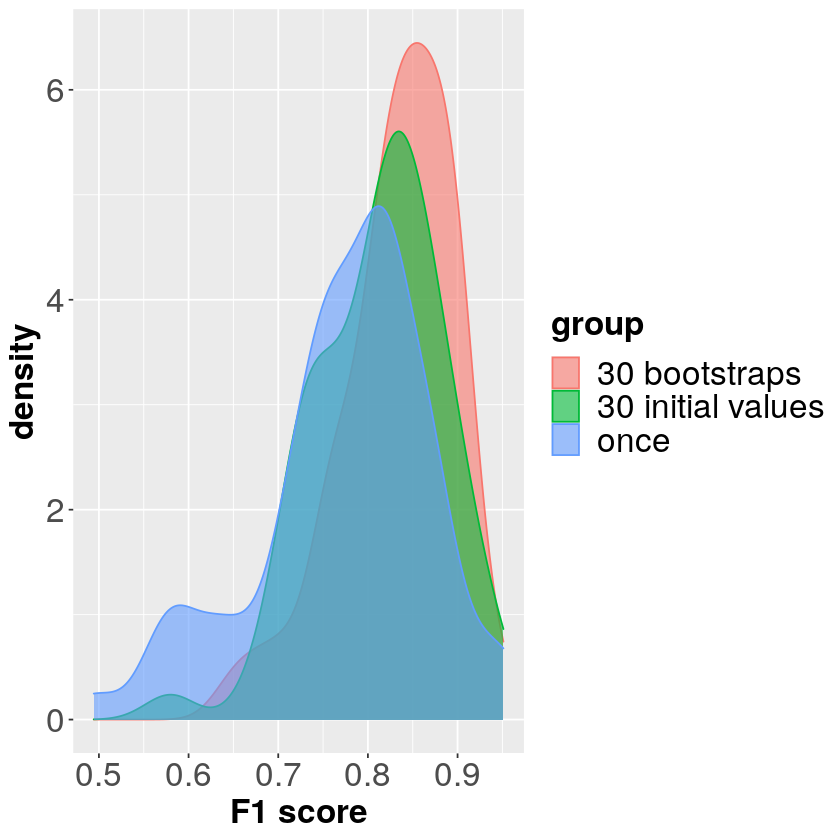
\includegraphics[width=\hsize]{once-init-boot}
					\caption{NMFを1回行った時の$A$,30回初期値を変えた$A$の平均,30回ブートストラップを行った$A$の平均それぞれのF1 scoreの分布.}
					\label{fig:once-init-boot}
			\end{center}
		\end{minipage}
    \begin{minipage}{0.5\hsize}
			\begin{center}
					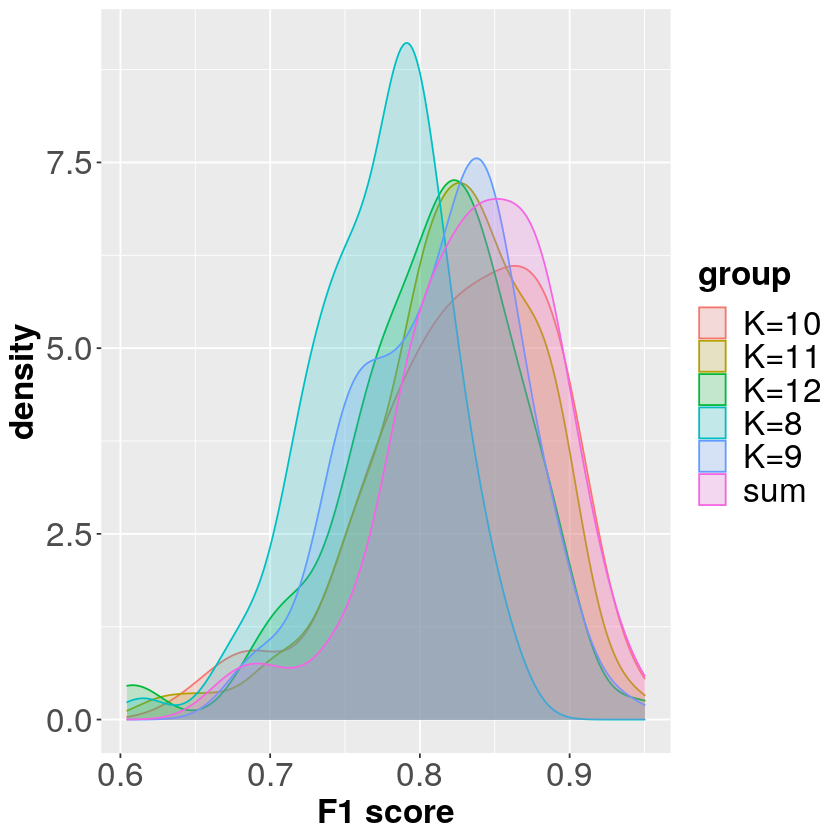
\includegraphics[width=\hsize]{f1all}
					\caption{基底数ごとにブートストラップを行った時の$A$のF1 scoreと全ての$A$の平均をとった時のF1 scoreの分布.}
					\label{fig:f1all}
			\end{center}
		\end{minipage}
\end{figure}
\Figref{fig:once-init-boot}より,ブートストラップを行った方が精度がよくなることがわかる.

基底数別に推定された$A$の平均をとった時のF1 scoreを~\Figref{fig:f1all}に示す.
これより,真の基底数周りの$A$の平均をとることである程度の精度は保たれることがわかる.

\subsection{NMFの基底数}
NMFの基底数を決める方法をいくつか試した.
人工データ86個についてBrunetらとUbrauらの方法で基底数を決めた時に各基底数が何回選ばれるかを~\Figref{fig:cophenetic}.\Figref{fig:uoi}に示す.
Brunetらの方法では真の基底数10に近い基底数が選ばれているが,Ubaruらの方法では小さい基底数が選ばれる傾向にあった.

また,1つの人工データについてAICとAICcを計算した結果を~\Figref{fig:aic},\Figref{fig:aicc}に示す.
どちらも基底数が大きくなるごとに減少する傾向があった.
他の人工データについても同様の結果であった.

\begin{figure}[htbp]
    \begin{minipage}{0.5\hsize}
        \begin{center}
            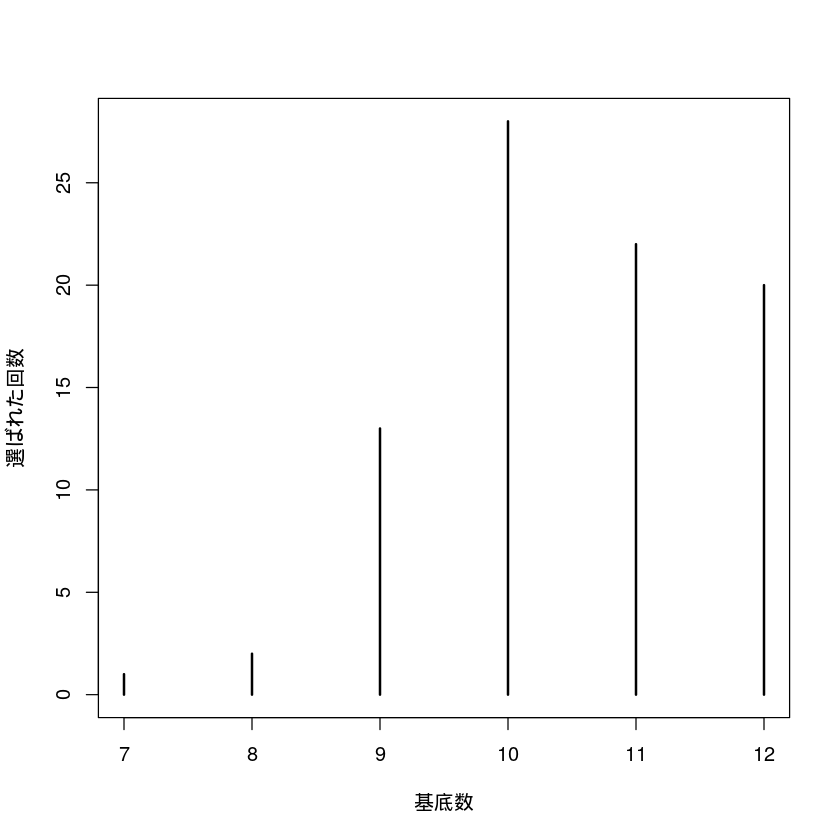
\includegraphics[width=\hsize]{cophenetic}
						\caption{Brunetらの方法で基底数を決めた時に各基底数が選ばれた回数(真の基底数は10).}
            \label{fig:cophenetic}
        \end{center}
    \end{minipage}
    \begin{minipage}{0.5\hsize}
        \begin{center}
            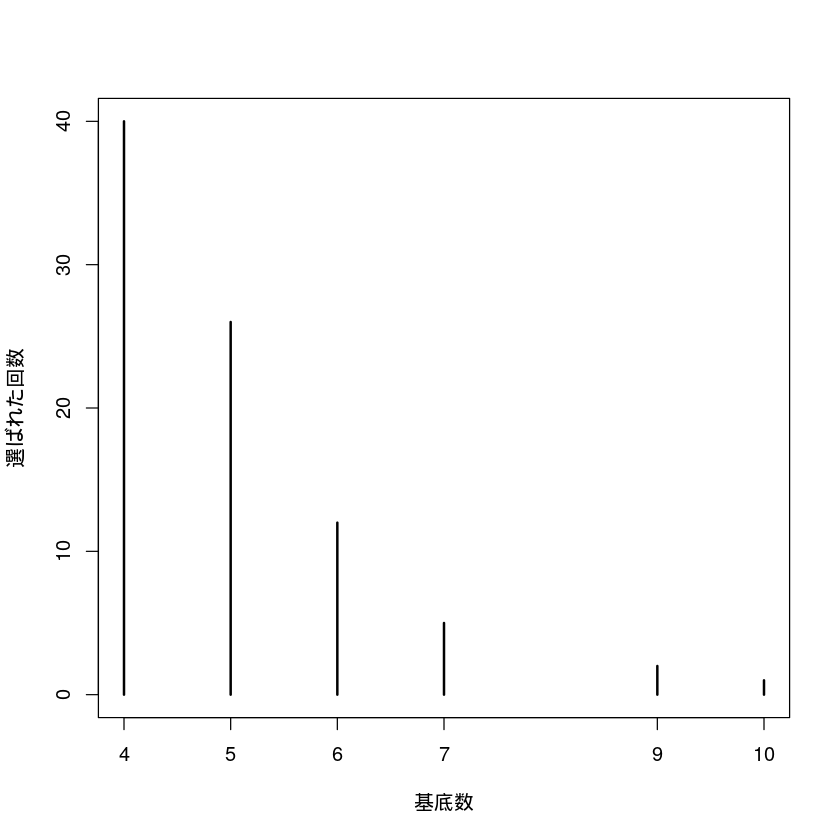
\includegraphics[width=\hsize]{uoi}
						\caption{Ubaruらの方法で基底数を決めた時に各基底数が選ばれた回数(真の基底数は10).}
            \label{fig:uoi}
        \end{center}
    \end{minipage}
\end{figure}
\begin{figure}[htbp]
    \begin{minipage}{0.5\hsize}
        \begin{center}
            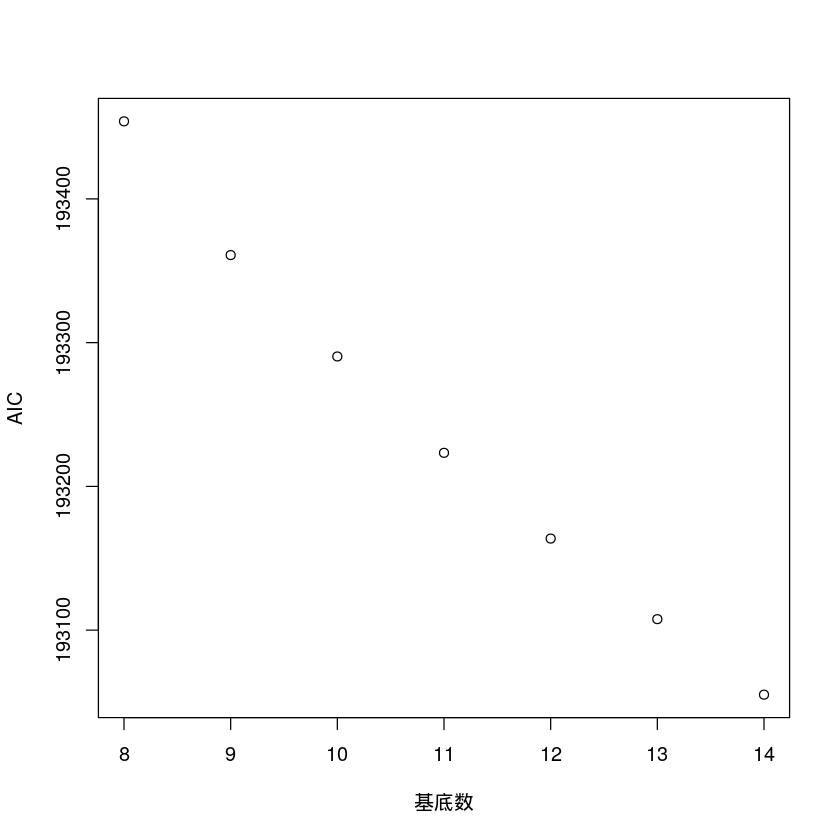
\includegraphics[width=\hsize]{aic}
						\caption{あるデータについてAICを計算した時の結果.}
            \label{fig:aic}
        \end{center}
    \end{minipage}
    \begin{minipage}{0.5\hsize}
        \begin{center}
						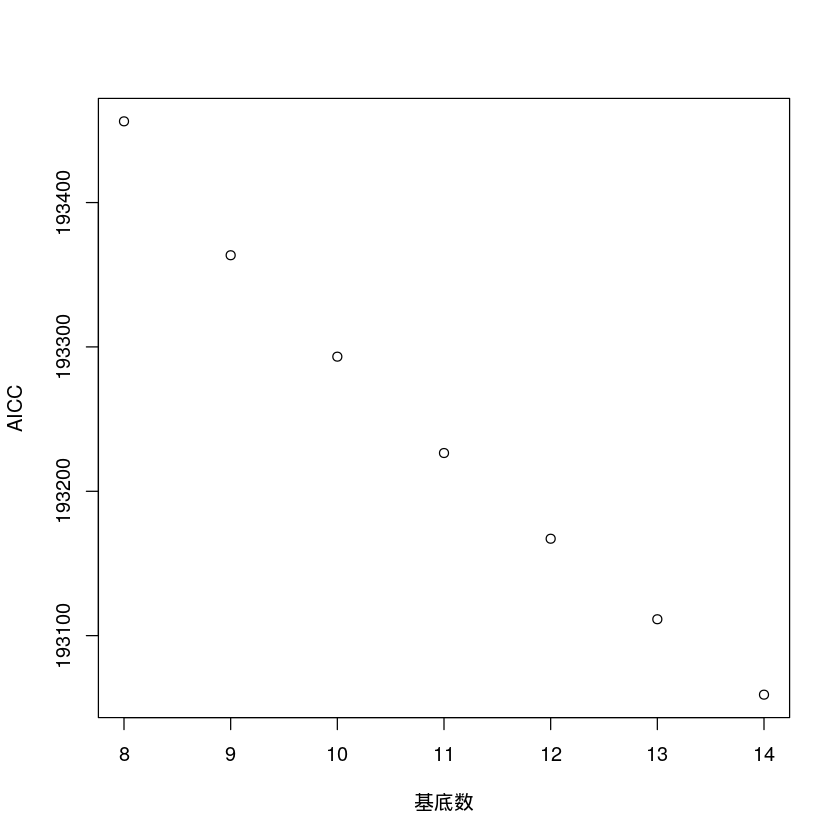
\includegraphics[width=\hsize]{aicc}
						\caption{あるデータについてAICc\cite{Symonds2011}を計算した時の結果.}
            \label{fig:aicc}
        \end{center}
    \end{minipage}
\end{figure}

\section{$A$のクラスタリングに関する結果}
\subsection{クラスタ数の決定}
スペクトラルクラスタリングでクラスタ数を決定する方法はいくつかあるが,その中でも小さい固有値を見る方法と,Gap統計量を用いた方法を試す.
$A$と比較する類似度行列として,データの相互相関行列と分散共分散行列を用いる.
